\begin{figure}[h!]
    \centering
    \begin{subfigure}[t]{0.38\textwidth}
        \centering
        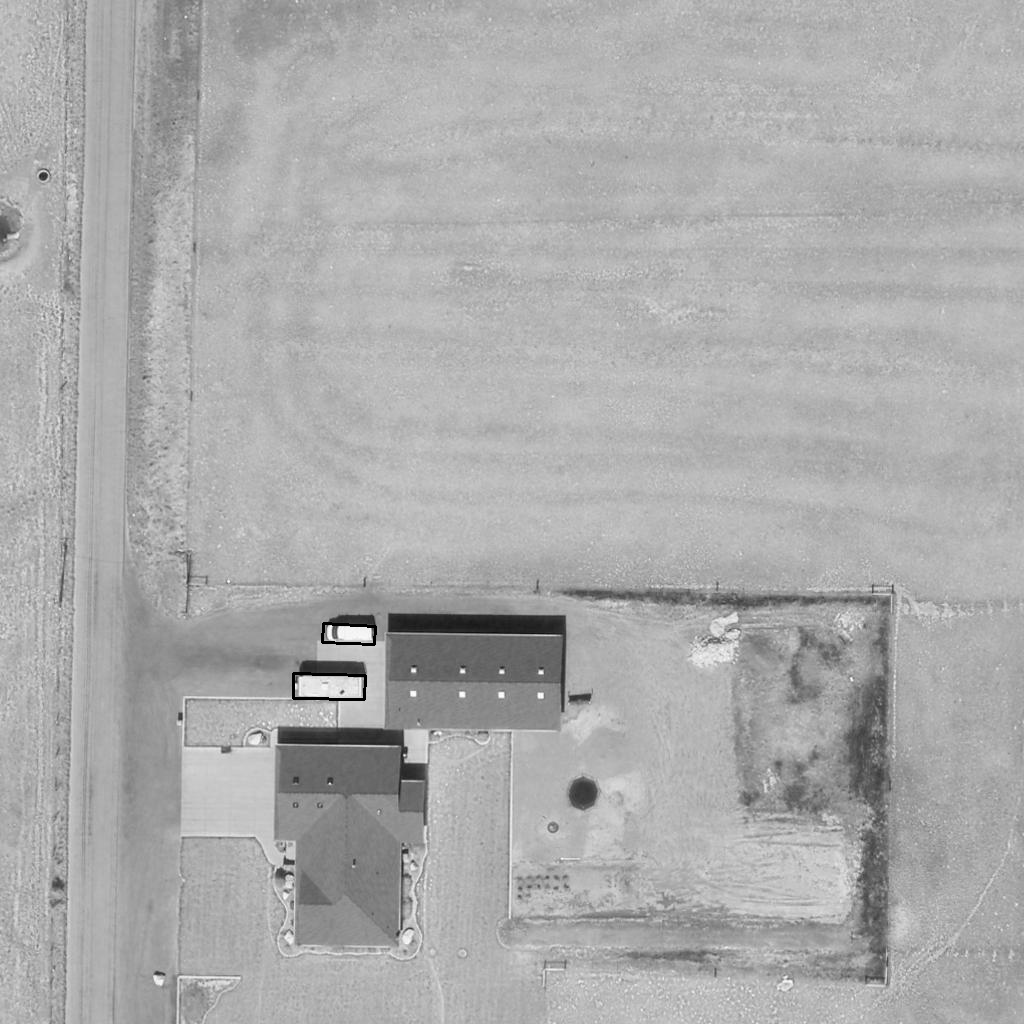
\includegraphics[width=\linewidth]{images/015Results/03ablation/comp_images/ground_truth/198.png}
        \caption{Van}
    \end{subfigure}
    \begin{subfigure}[t]{0.38\textwidth}
        \centering
        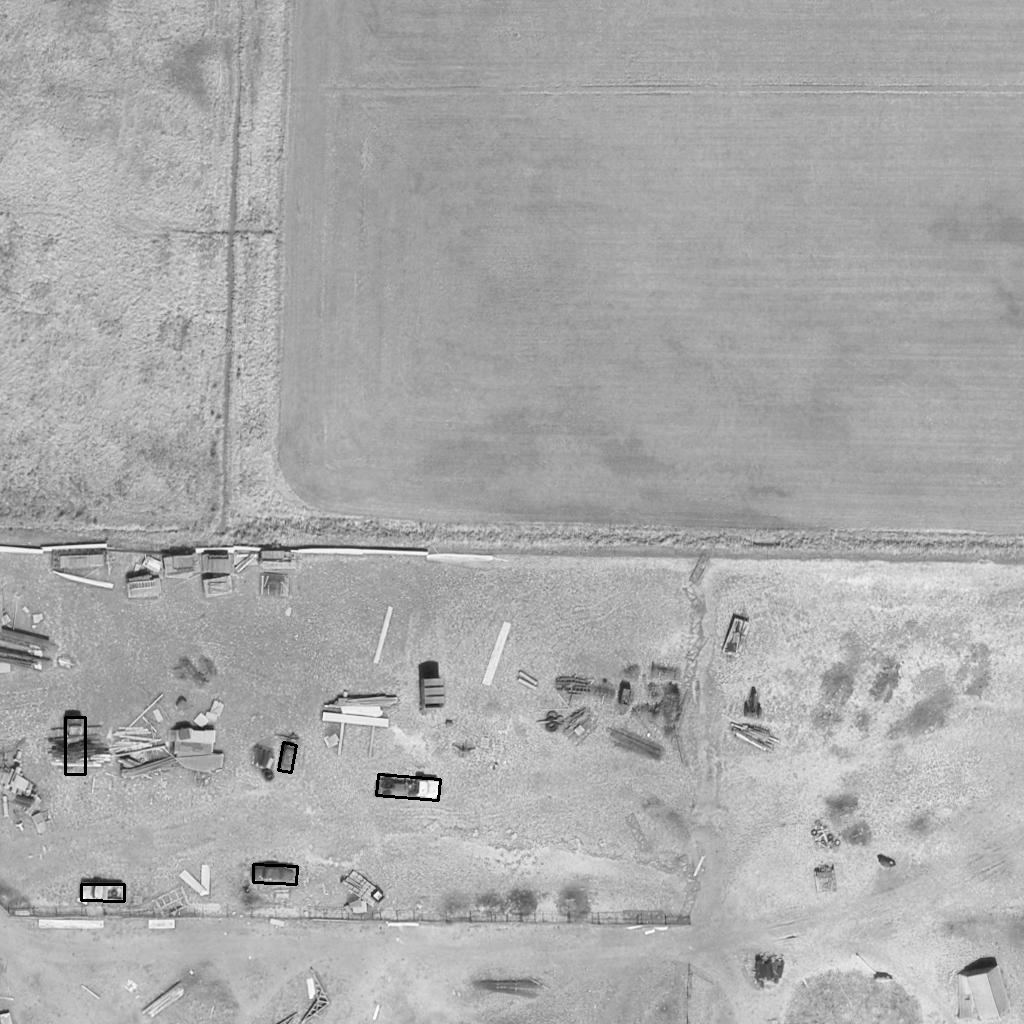
\includegraphics[width=\linewidth]{images/015Results/03ablation/comp_images/ground_truth/212.png}
        \caption{Truck}
    \end{subfigure}
    
    \begin{subfigure}[t]{0.38\textwidth}
        \centering
        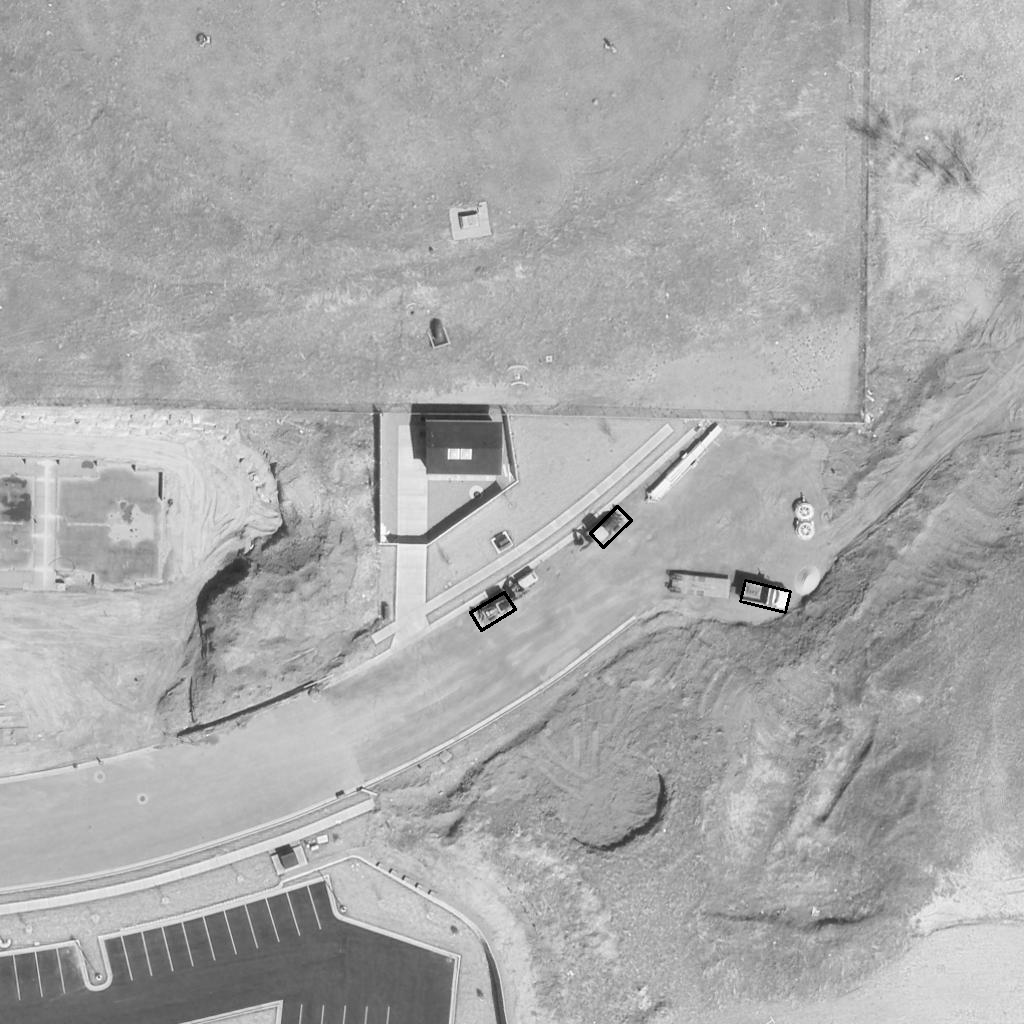
\includegraphics[width=\linewidth]{images/015Results/03ablation/comp_images/ground_truth/427.png}
        \caption{Vehicle}
    \end{subfigure}
    \begin{subfigure}[t]{0.38\textwidth}
        \centering
        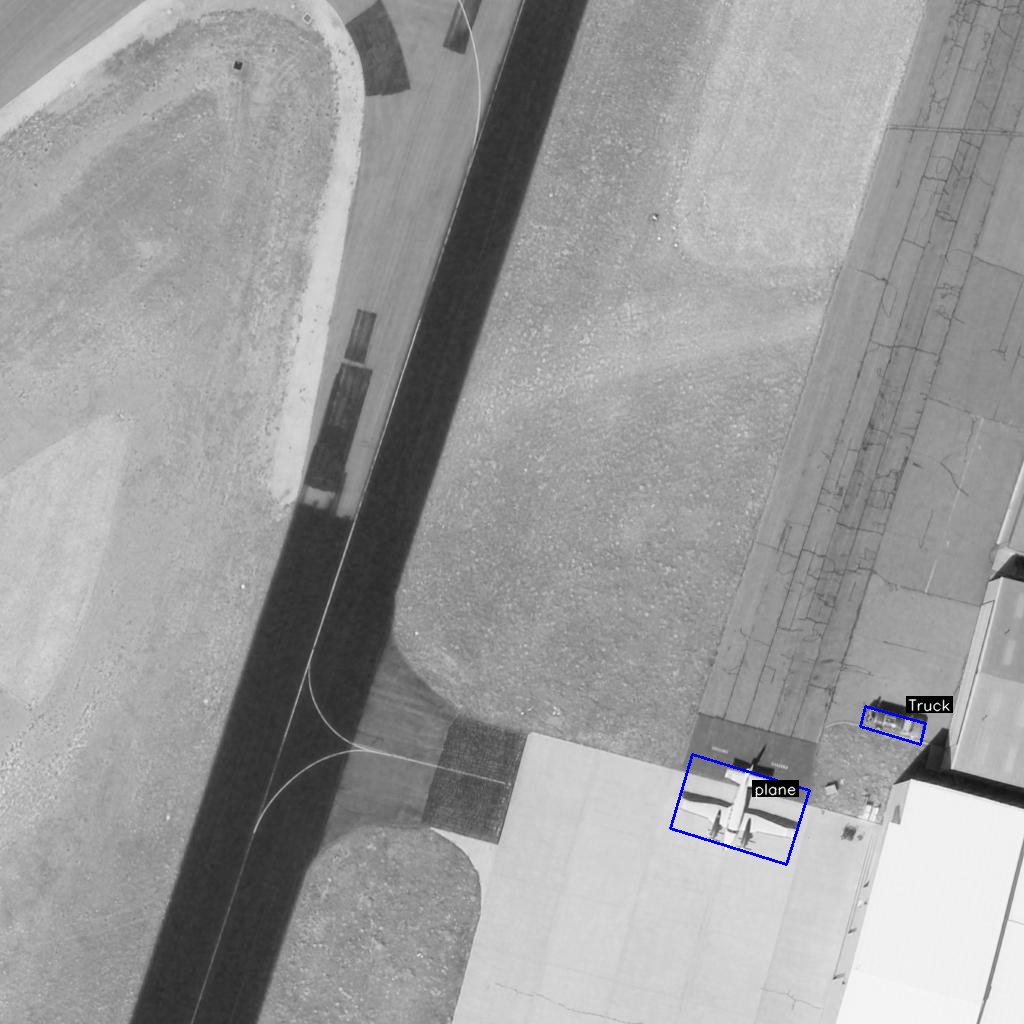
\includegraphics[width=\linewidth]{images/015Results/03ablation/comp_images/ground_truth/487.png}
        \caption{Plane}
    \end{subfigure}
    
    \begin{subfigure}[t]{0.38\textwidth}
        \centering
        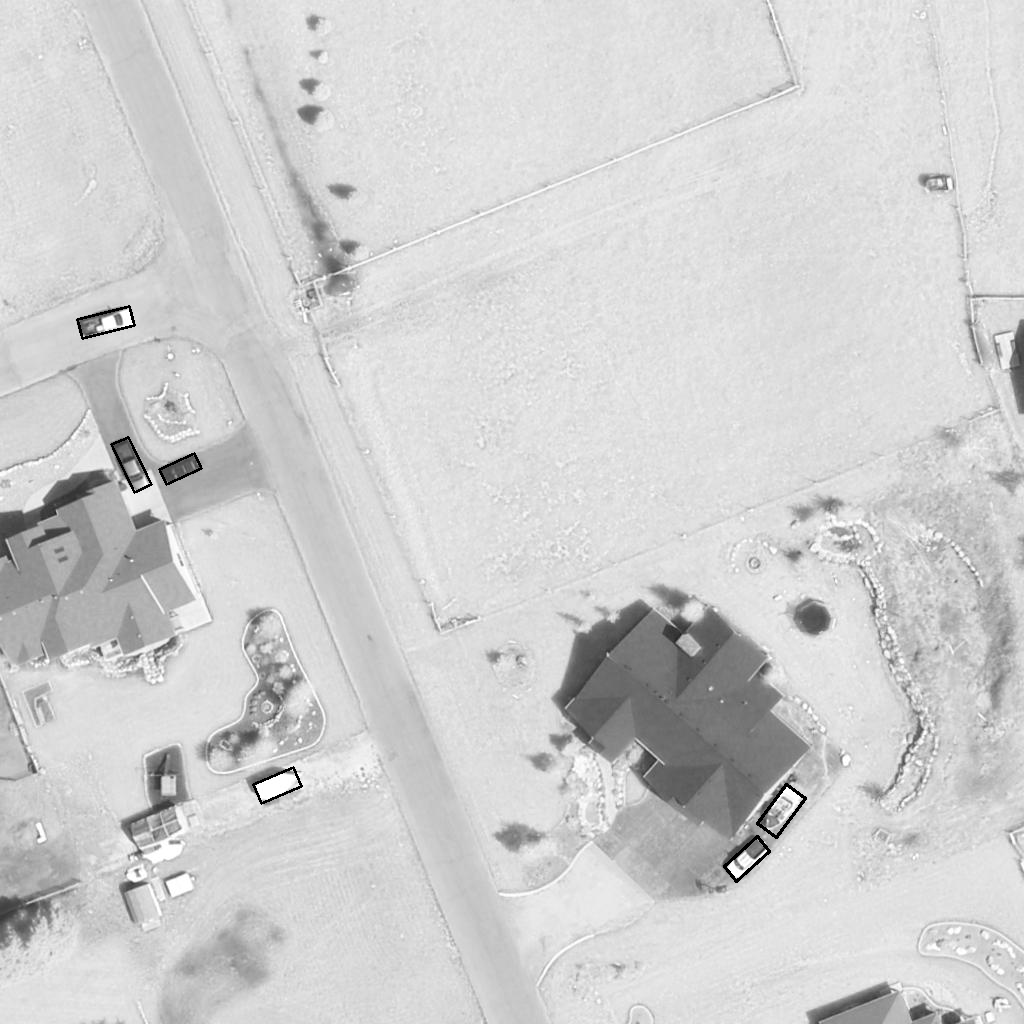
\includegraphics[width=\linewidth]{images/015Results/03ablation/comp_images/ground_truth/509.png}
        \caption{Ship}
    \end{subfigure}
    \begin{subfigure}[t]{0.38\textwidth}
        \centering
        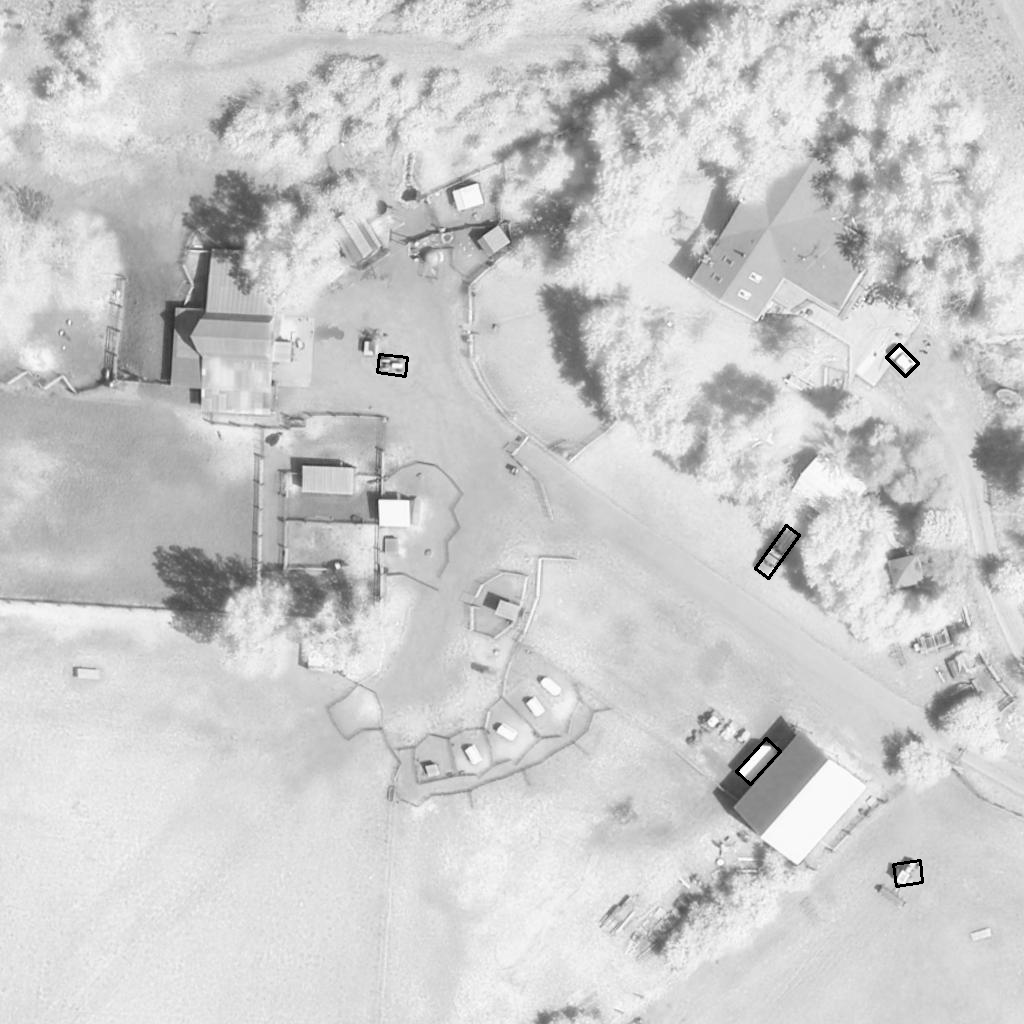
\includegraphics[width=\linewidth]{images/015Results/03ablation/comp_images/ground_truth/523.png}
        \caption{Car, Tractor, Pick-Up}
    \end{subfigure}
    
    \caption[Ground Truth (Ablation Studies) – Full Sized Images]{Ground Truth (Ablation Studies) – Full Sized Images. The captions below the partial illustrations correspond to the classes shown in the example images. However, the illustrations generally show more classes than are indicated in the captions.}
    \label{fig:gt_ablation_examples_fs}
\end{figure}



\begin{figure}[h!]
    \centering
    \begin{subfigure}[t]{0.38\textwidth}
        \centering
        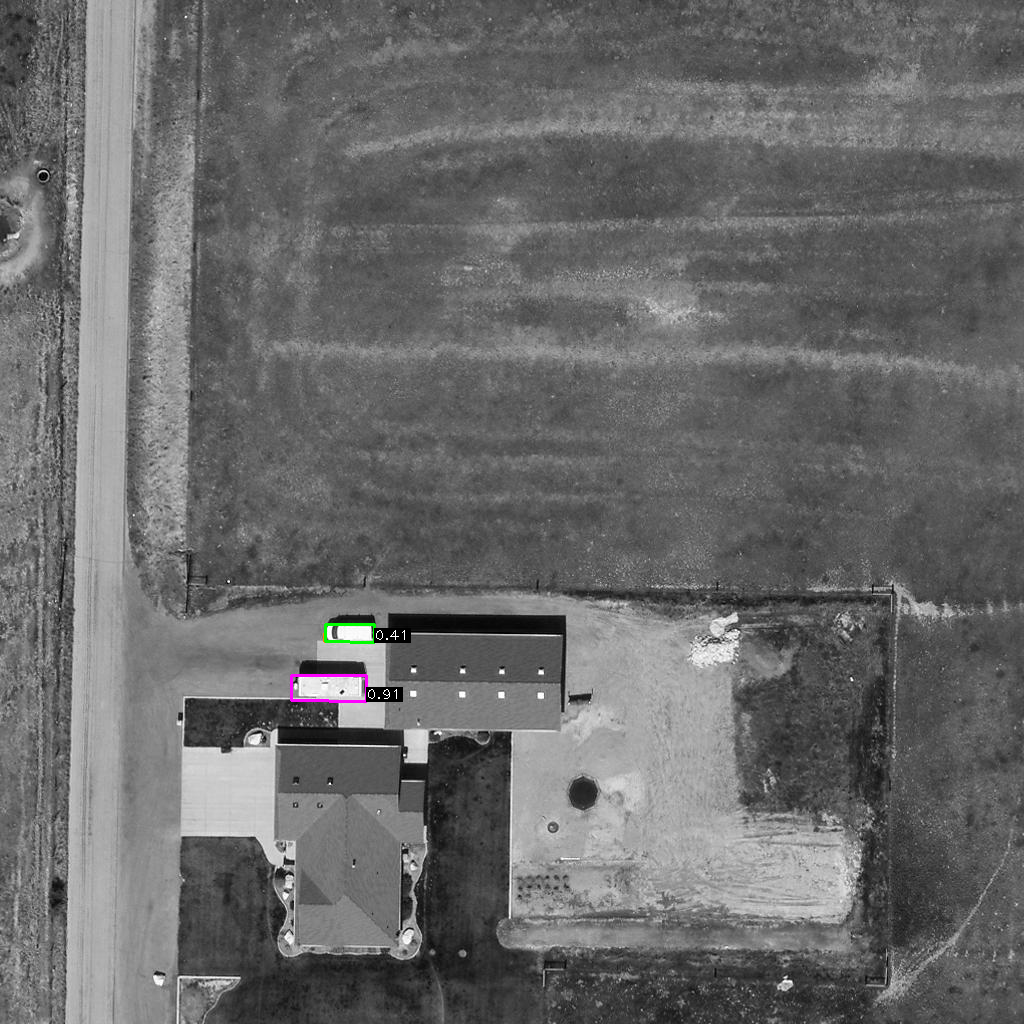
\includegraphics[width=\linewidth]{images/015Results/03ablation/comp_images/red/198.png}
        \caption{Van}
    \end{subfigure}
    \begin{subfigure}[t]{0.38\textwidth}
        \centering
        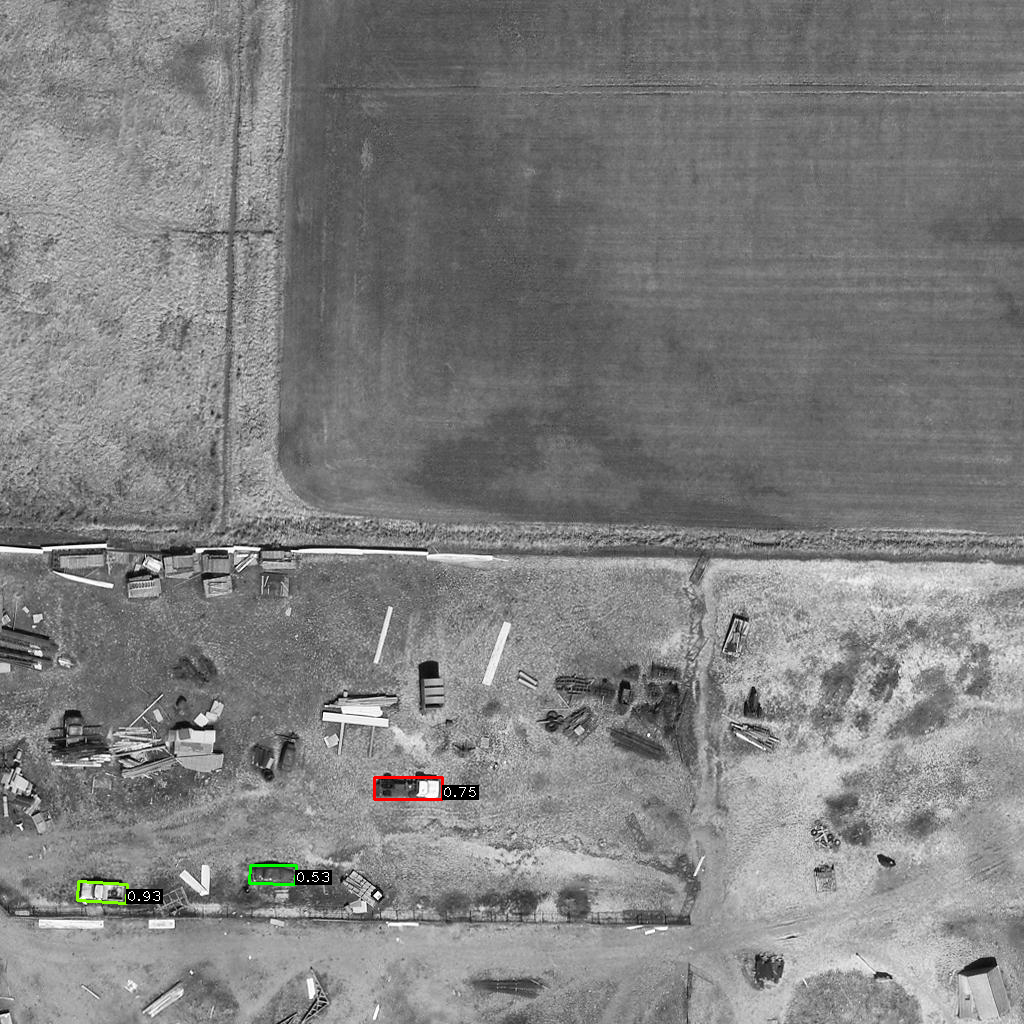
\includegraphics[width=\linewidth]{images/015Results/03ablation/comp_images/red/212.png}
        \caption{Truck}
    \end{subfigure}
    
    \begin{subfigure}[t]{0.38\textwidth}
        \centering
        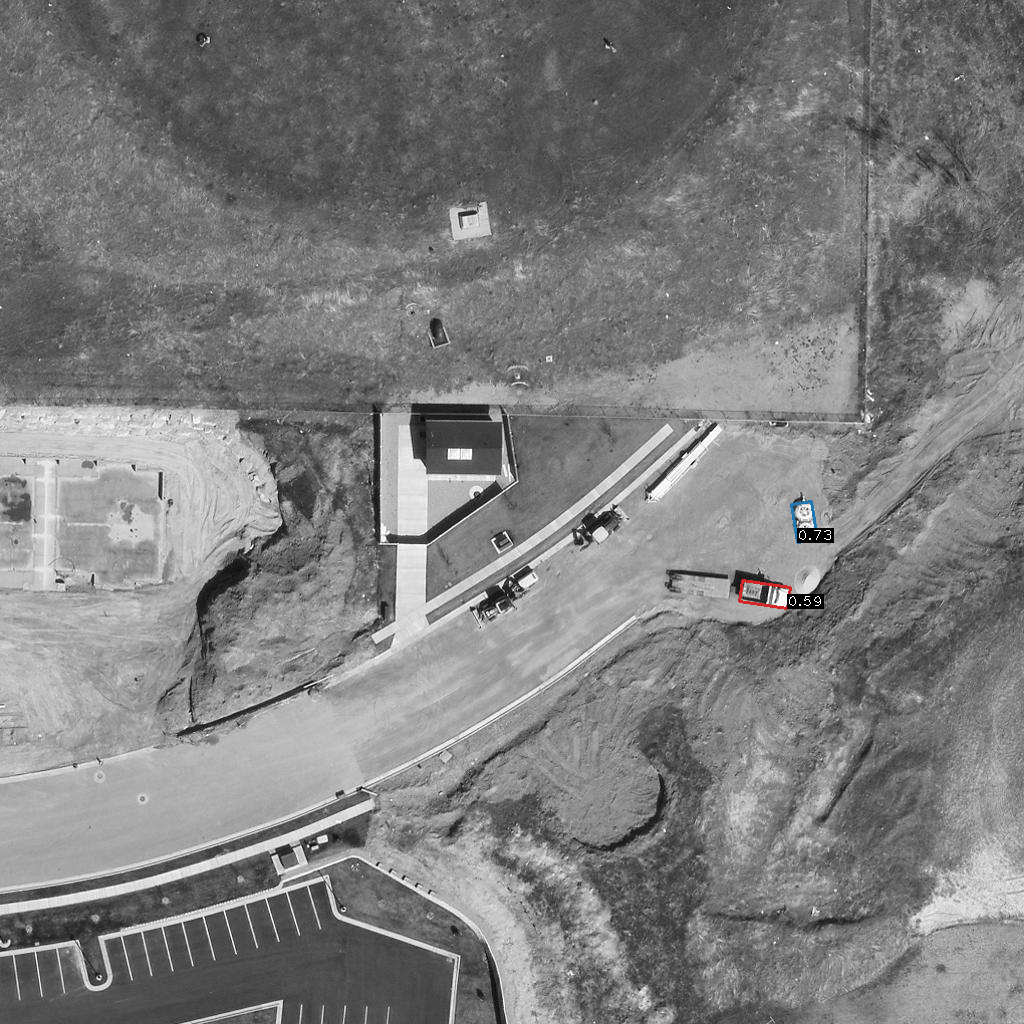
\includegraphics[width=\linewidth]{images/015Results/03ablation/comp_images/red/427.png}
        \caption{Vehicle}
    \end{subfigure}
    \begin{subfigure}[t]{0.38\textwidth}
        \centering
        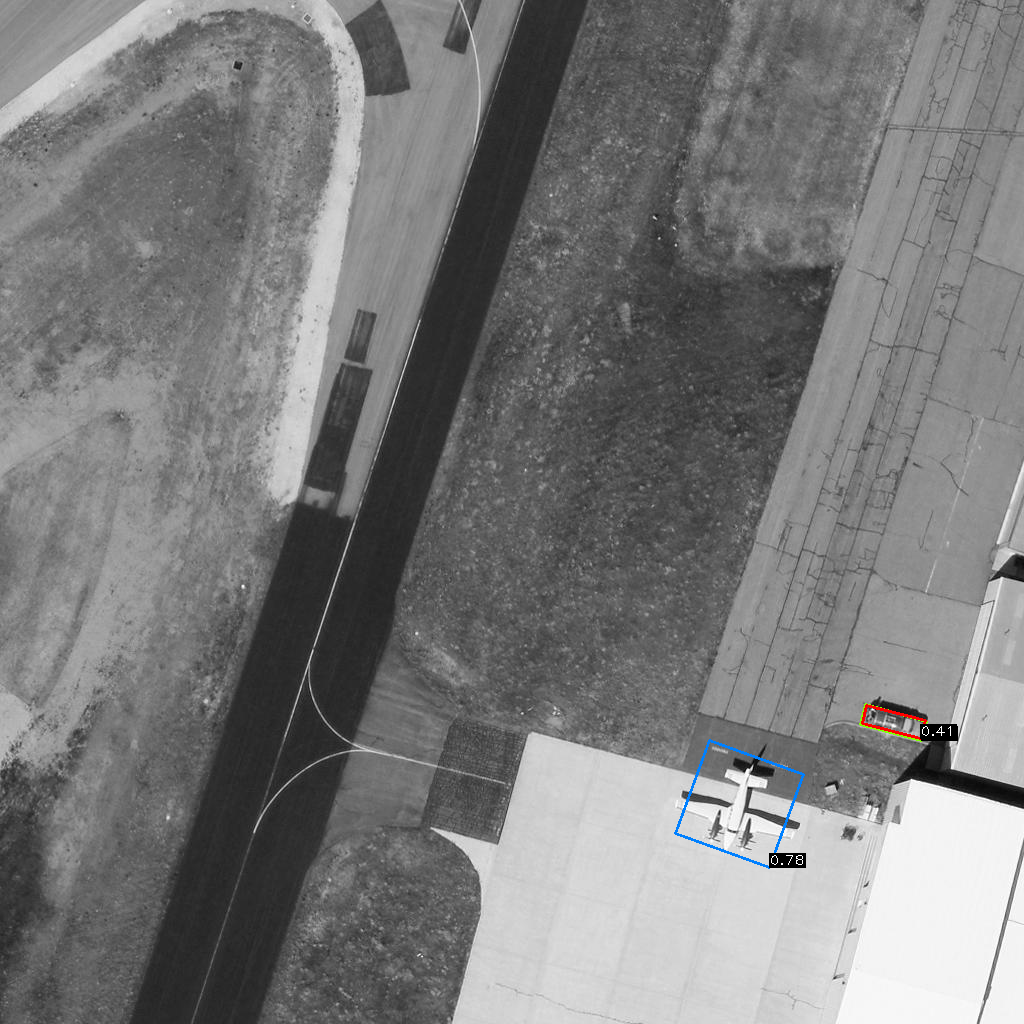
\includegraphics[width=\linewidth]{images/015Results/03ablation/comp_images/red/487.png}
        \caption{Plane}
    \end{subfigure}
    
    \begin{subfigure}[t]{0.38\textwidth}
        \centering
        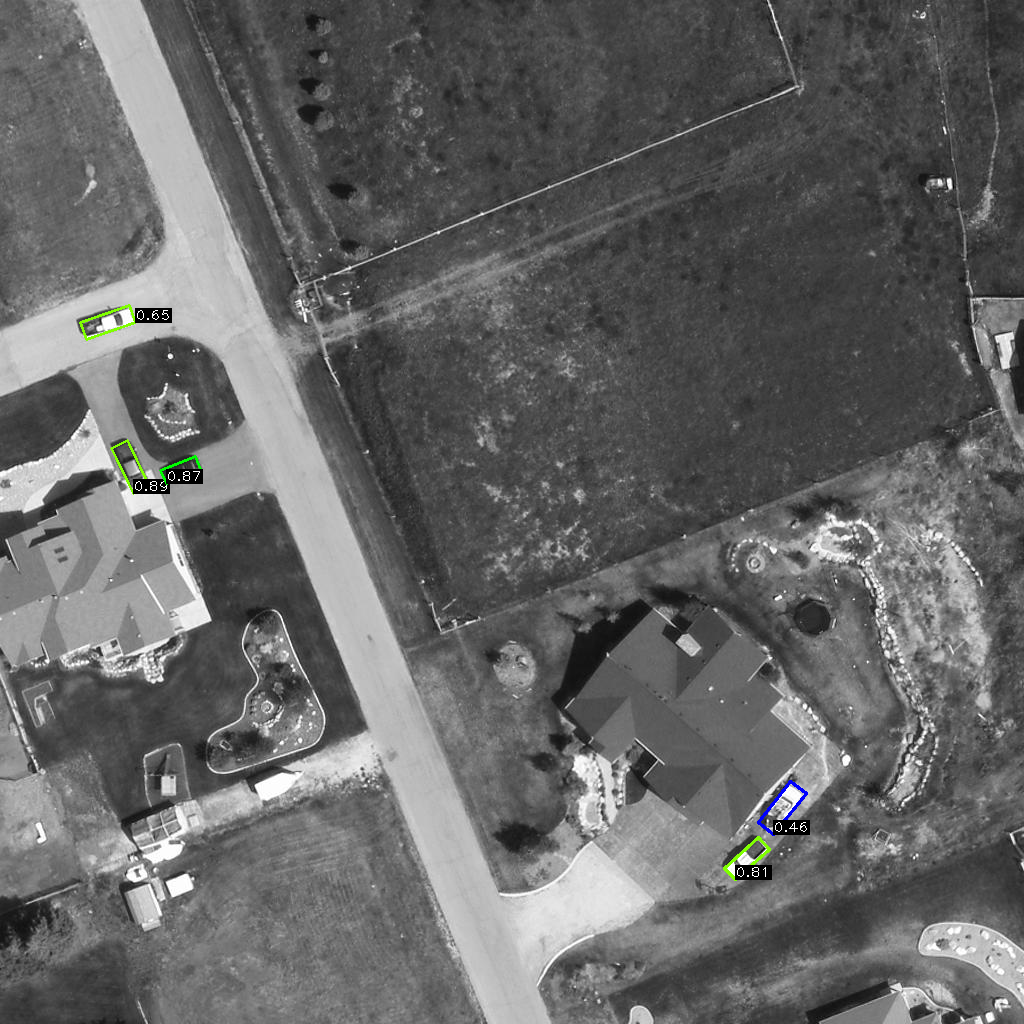
\includegraphics[width=\linewidth]{images/015Results/03ablation/comp_images/red/509.png}
        \caption{Ship}
    \end{subfigure}
    \begin{subfigure}[t]{0.38\textwidth}
        \centering
        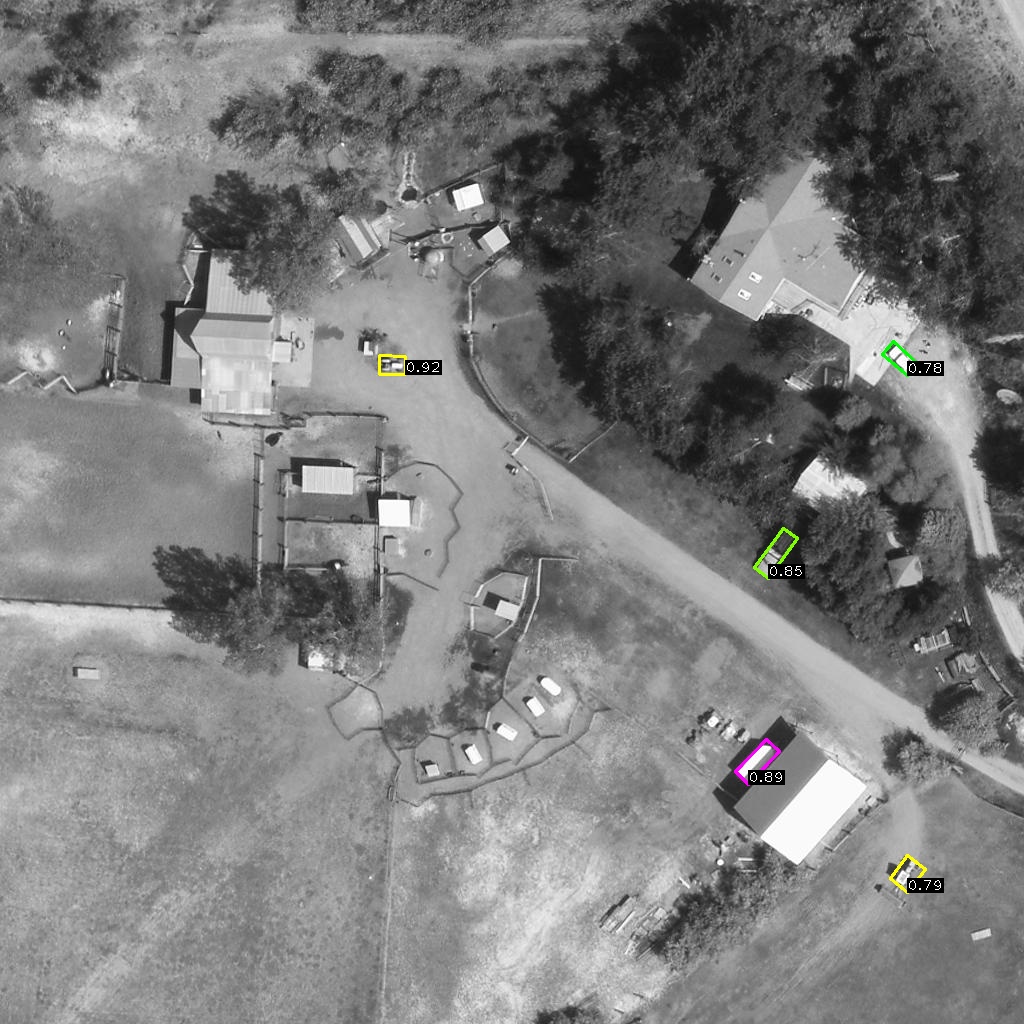
\includegraphics[width=\linewidth]{images/015Results/03ablation/comp_images/red/523.png}
        \caption{Car, Tractor, Pick-Up}
    \end{subfigure}
    
    \caption[Red Model – Full Sized Images]{Red Model – Full Sized Images. The captions below the partial illustrations correspond to the classes shown in the example images. However, the illustrations generally show more classes than are indicated in the captions.}
    \label{fig:red_ablation_examples_fs}
\end{figure}

\begin{figure}[h!]
    \centering
    \begin{subfigure}[t]{0.38\textwidth}
        \centering
        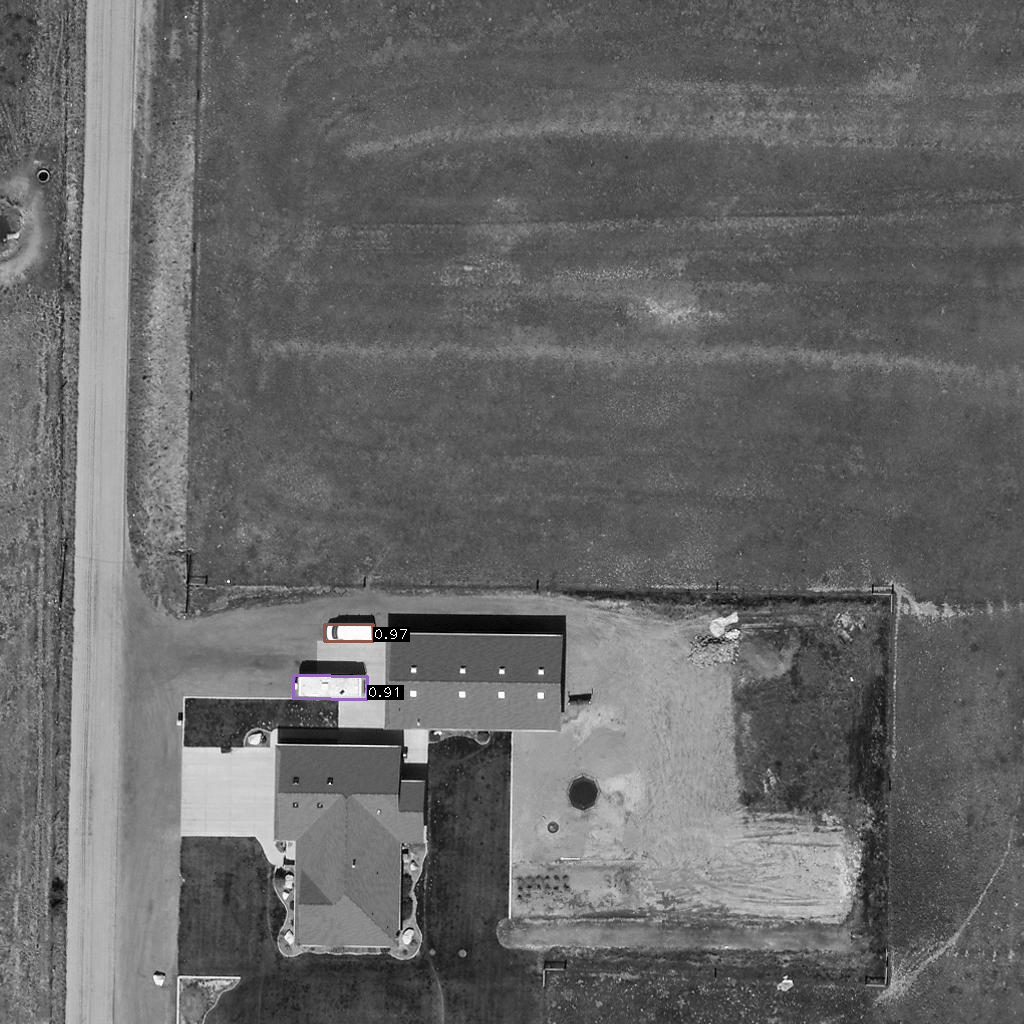
\includegraphics[width=\linewidth]{images/015Results/03ablation/comp_images/green/198.png}
        \caption{Van}
    \end{subfigure}
    \begin{subfigure}[t]{0.38\textwidth}
        \centering
        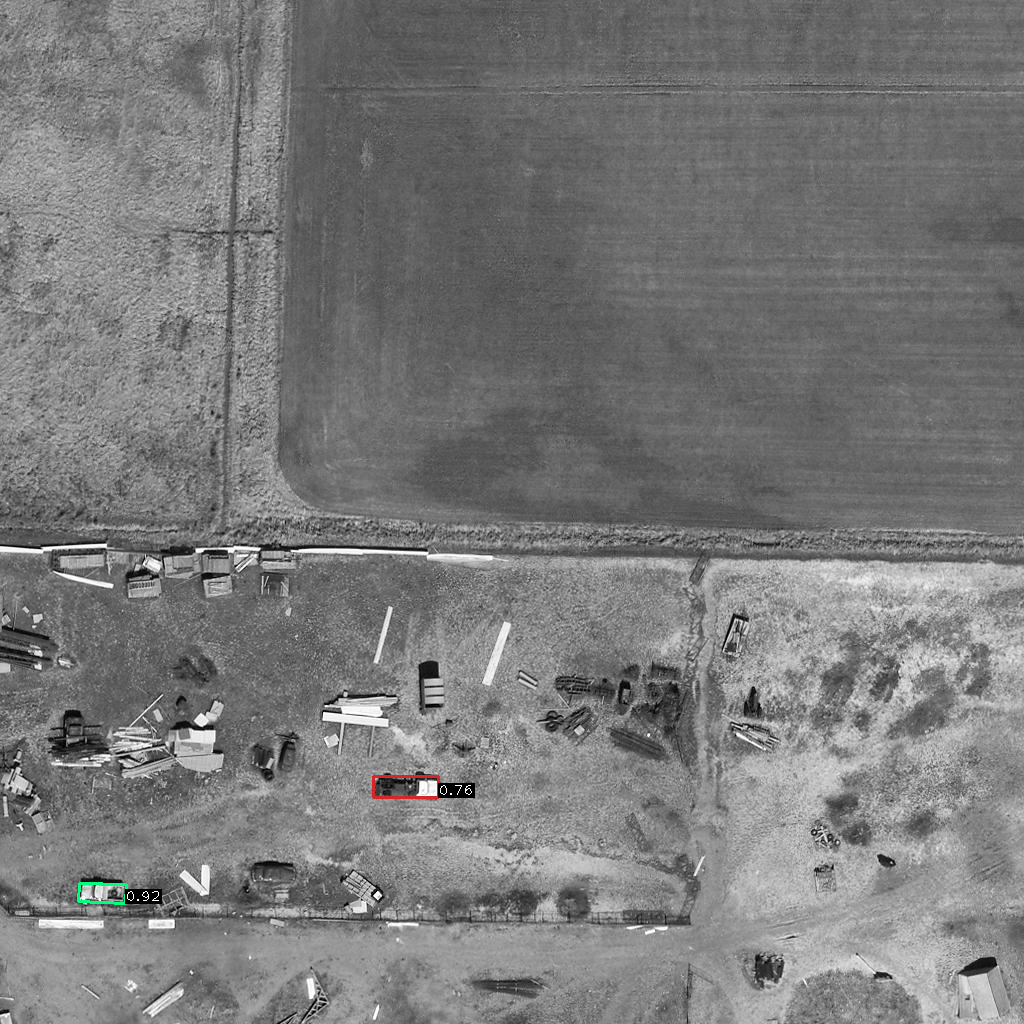
\includegraphics[width=\linewidth]{images/015Results/03ablation/comp_images/green/212.png}
        \caption{Truck}
    \end{subfigure}
    
    \begin{subfigure}[t]{0.38\textwidth}
        \centering
        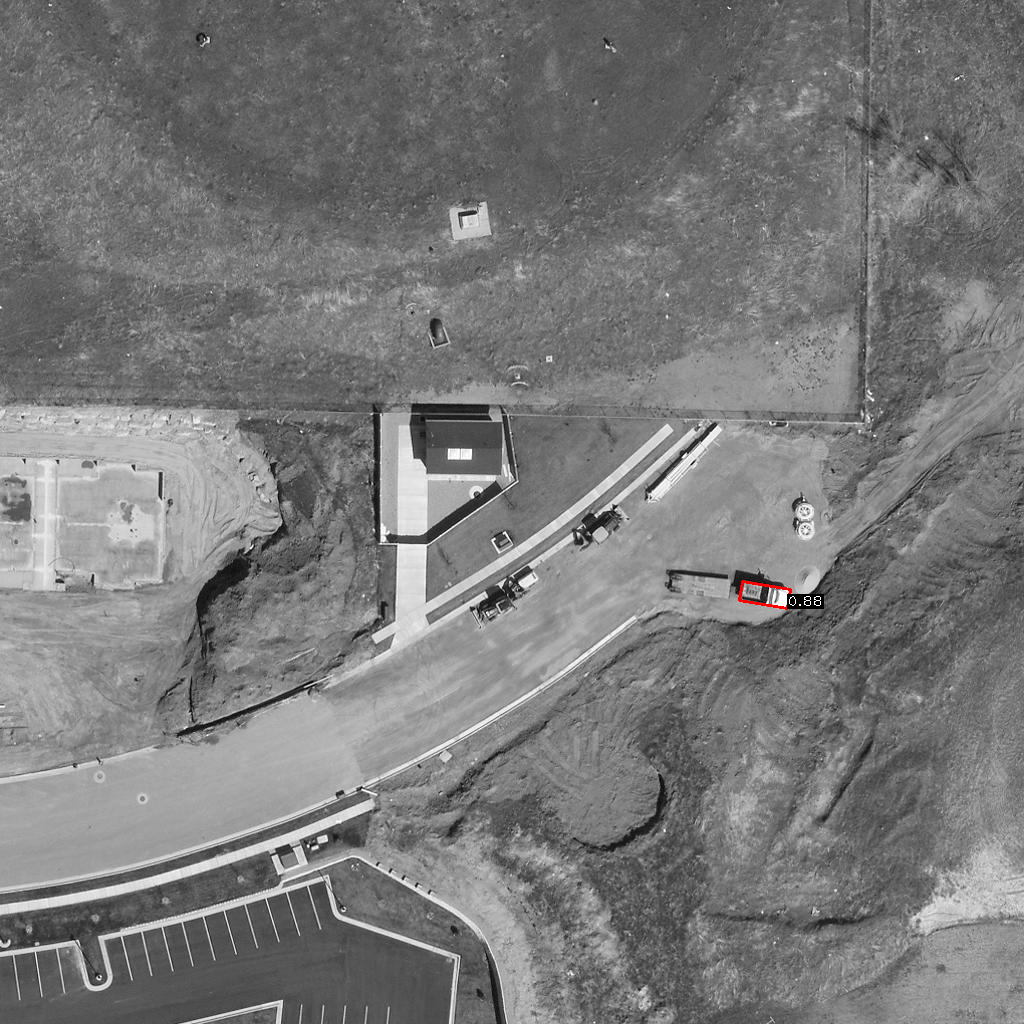
\includegraphics[width=\linewidth]{images/015Results/03ablation/comp_images/green/427.png}
        \caption{Vehicle}
    \end{subfigure}
    \begin{subfigure}[t]{0.38\textwidth}
        \centering
        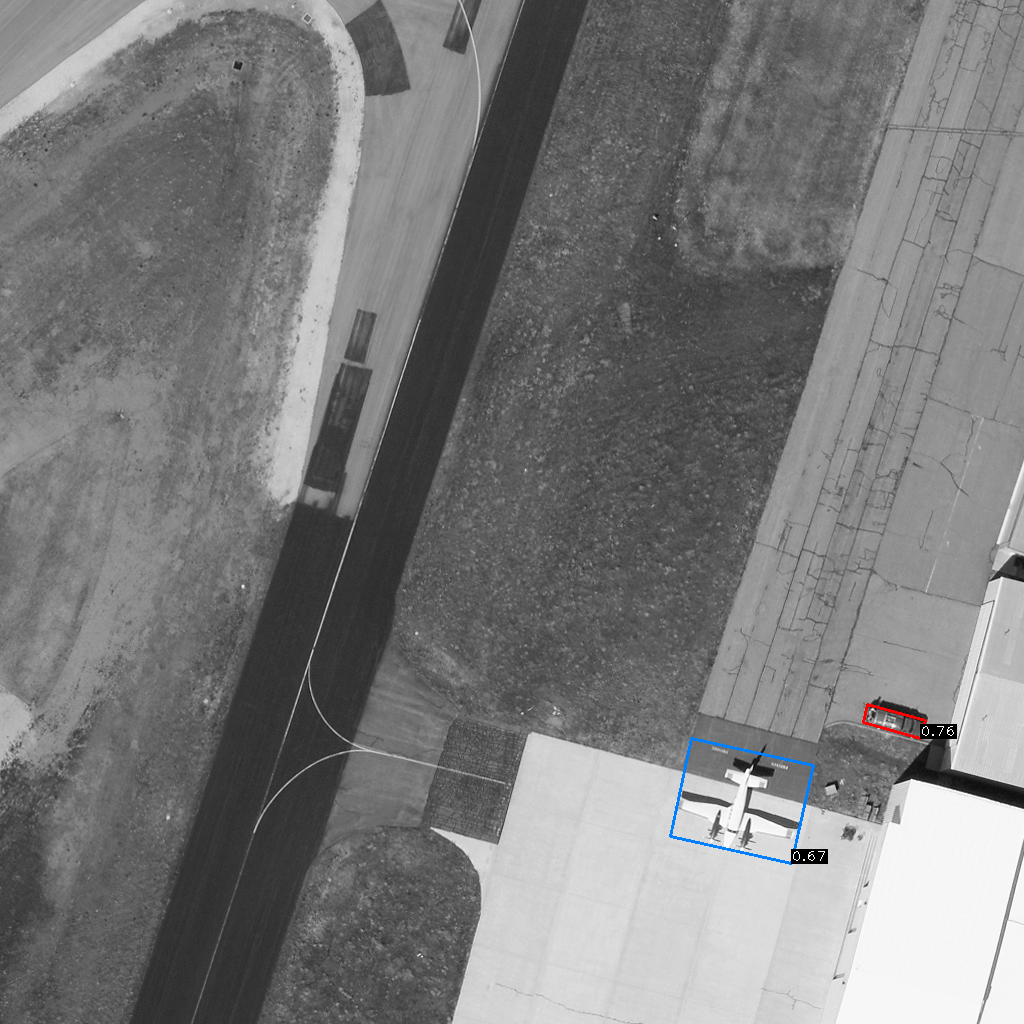
\includegraphics[width=\linewidth]{images/015Results/03ablation/comp_images/green/487.png}
        \caption{Plane}
    \end{subfigure}
    
    \begin{subfigure}[t]{0.38\textwidth}
        \centering
        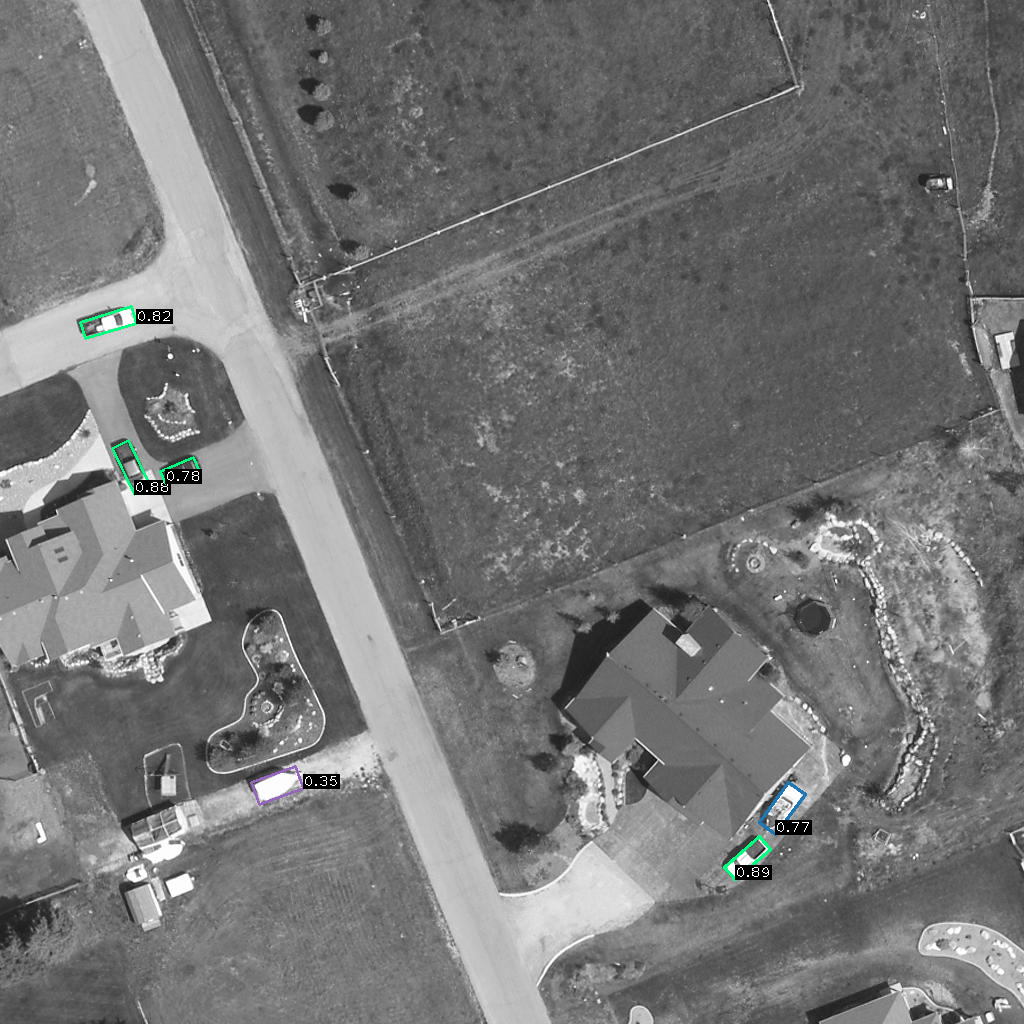
\includegraphics[width=\linewidth]{images/015Results/03ablation/comp_images/green/509.png}
        \caption{Ship}
    \end{subfigure}
    \begin{subfigure}[t]{0.38\textwidth}
        \centering
        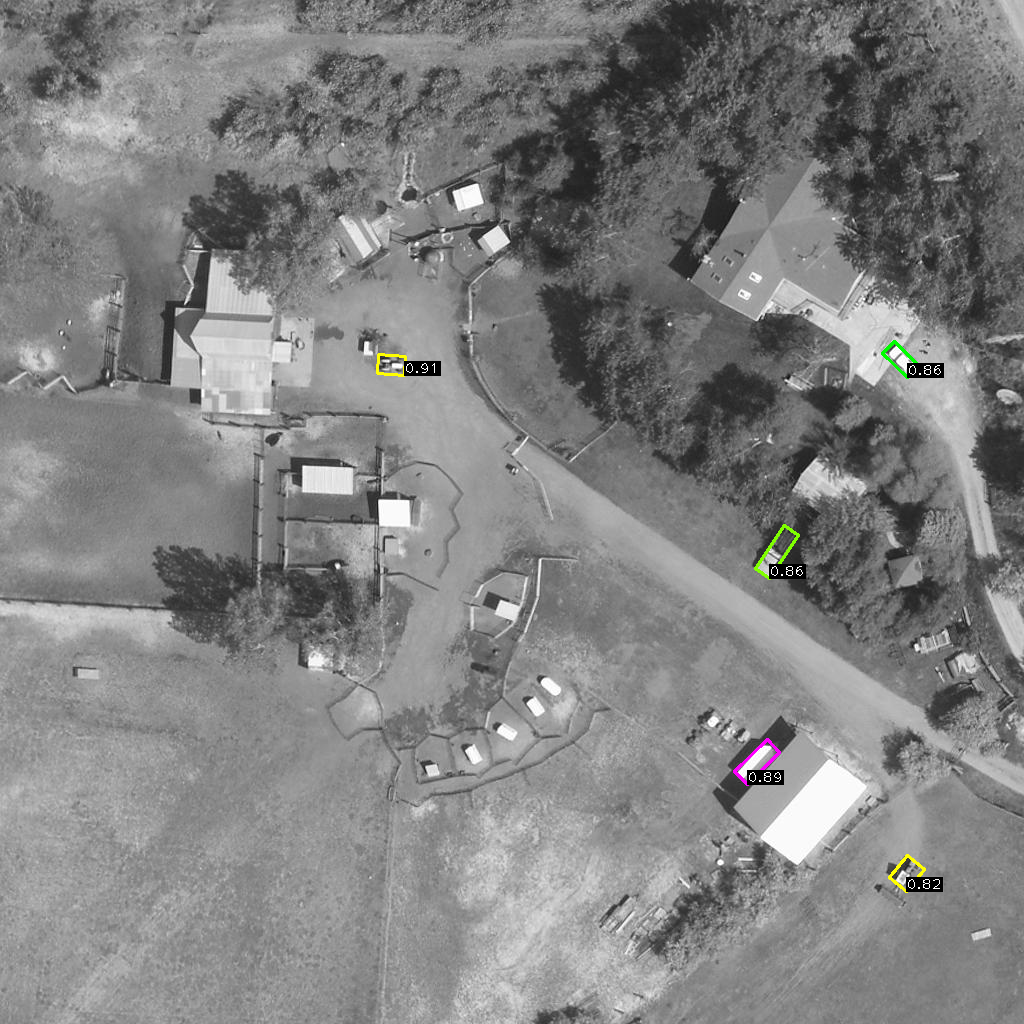
\includegraphics[width=\linewidth]{images/015Results/03ablation/comp_images/green/523.png}
        \caption{Car, Tractor, Pick-Up}
    \end{subfigure}
    
    \caption[Green Model – Full Sized Images]{Green Model – Full Sized Images. The captions below the partial illustrations correspond to the classes shown in the example images. However, the illustrations generally show more classes than are indicated in the captions.}
    \label{fig:green_ablation_examples_fs}
\end{figure}

\begin{figure}[h!]
    \centering
    \begin{subfigure}[t]{0.38\textwidth}
        \centering
        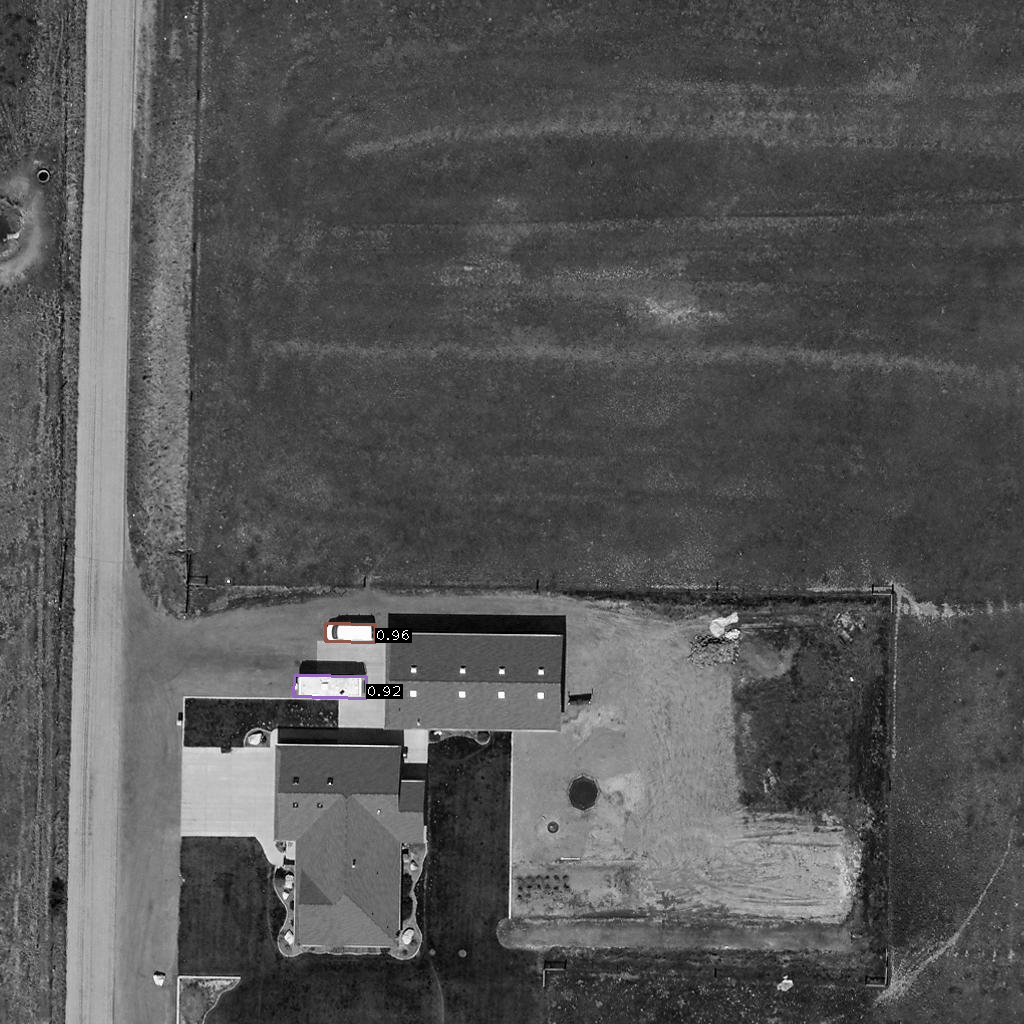
\includegraphics[width=\linewidth]{images/015Results/03ablation/comp_images/blue/198.png}
        \caption{Van}
    \end{subfigure}
    \begin{subfigure}[t]{0.38\textwidth}
        \centering
        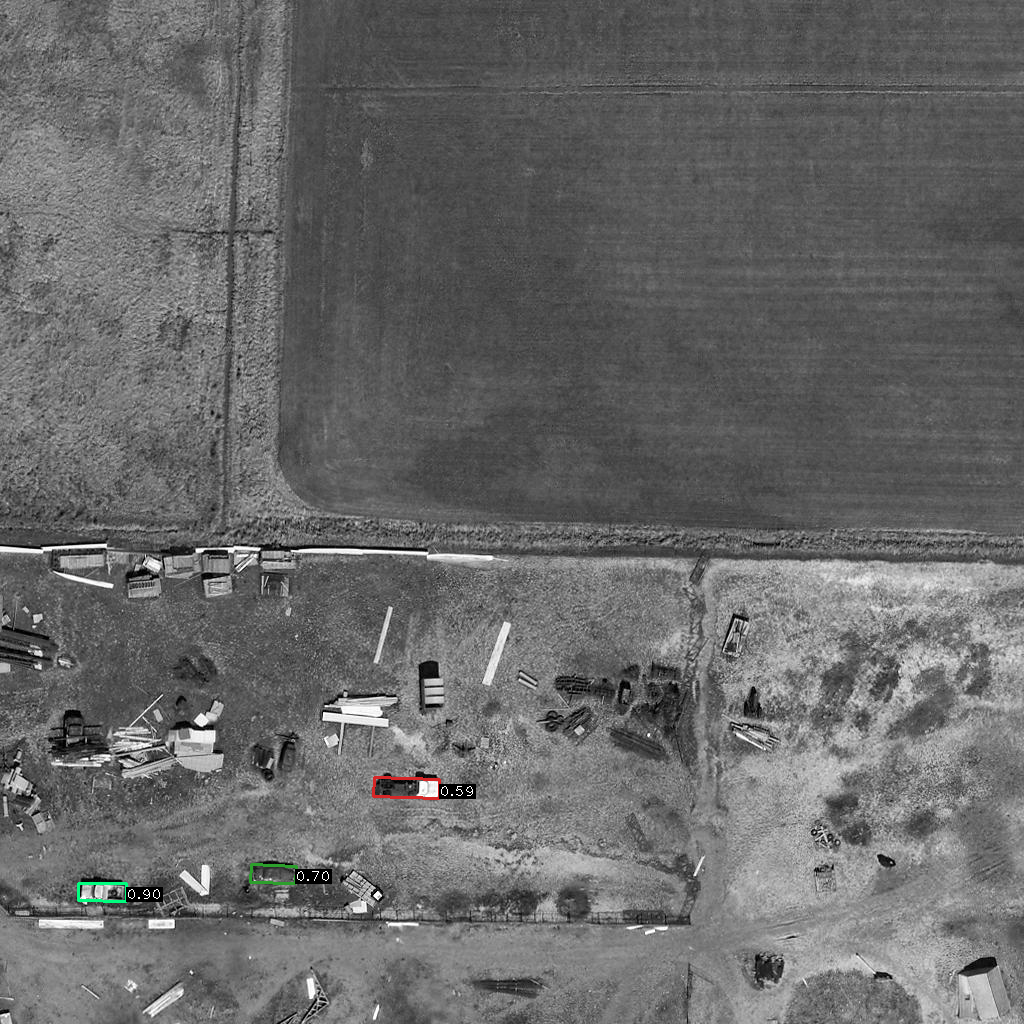
\includegraphics[width=\linewidth]{images/015Results/03ablation/comp_images/blue/212.png}
        \caption{Truck}
    \end{subfigure}
    
    \begin{subfigure}[t]{0.38\textwidth}
        \centering
        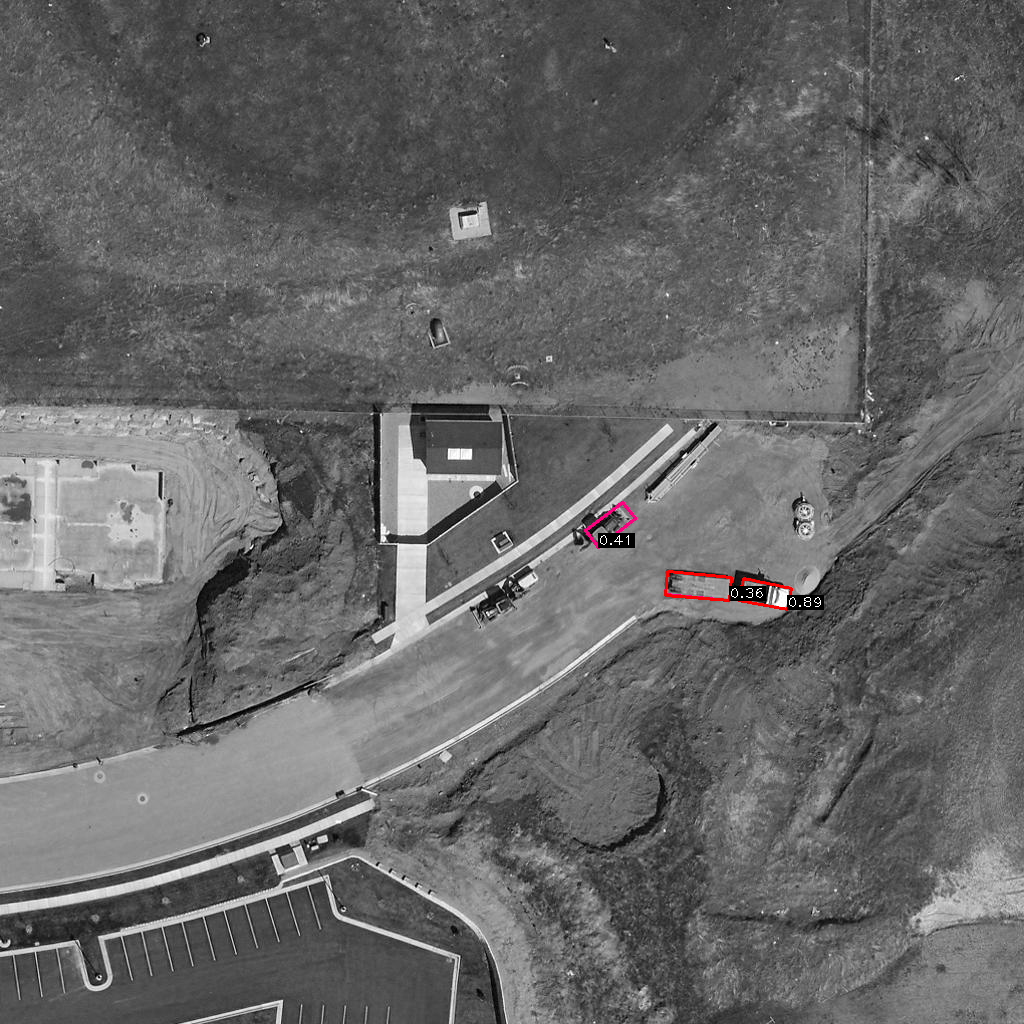
\includegraphics[width=\linewidth]{images/015Results/03ablation/comp_images/blue/427.png}
        \caption{Vehicle}
    \end{subfigure}
    \begin{subfigure}[t]{0.38\textwidth}
        \centering
        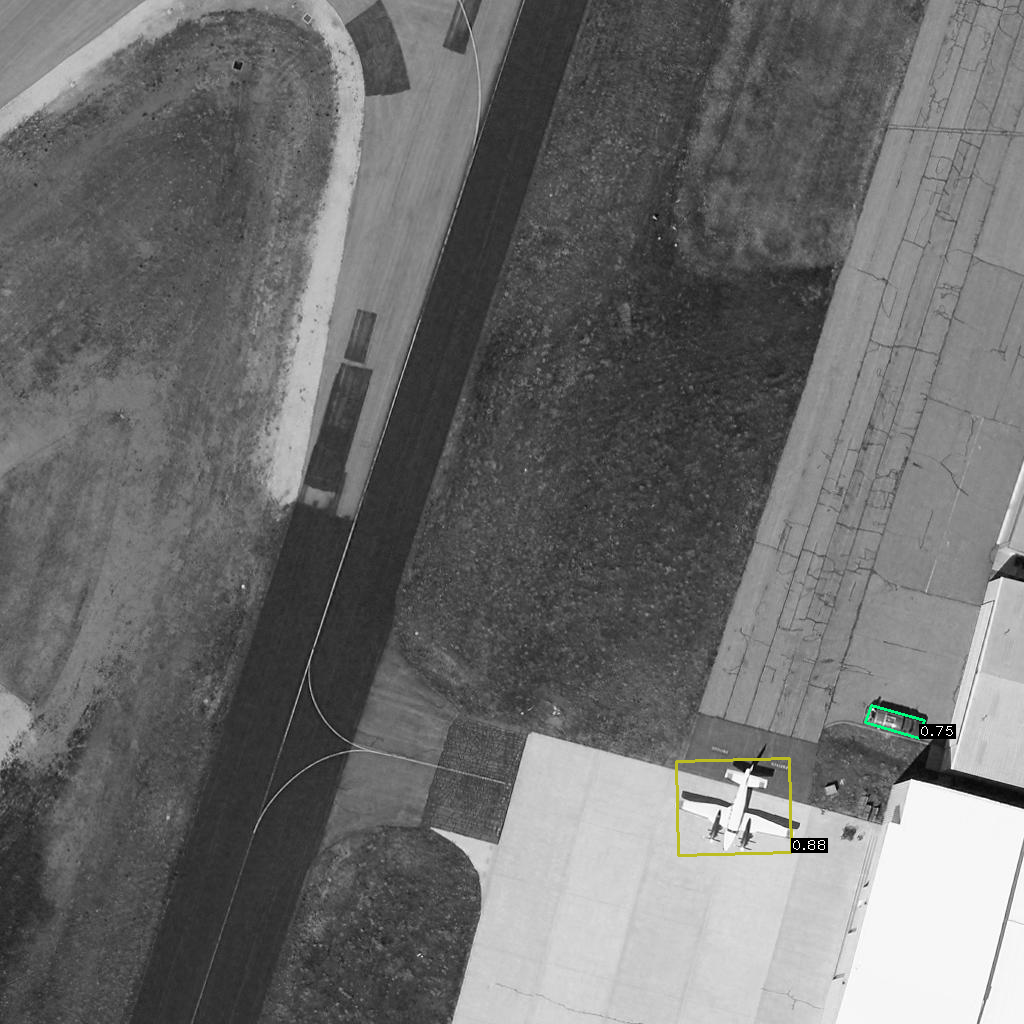
\includegraphics[width=\linewidth]{images/015Results/03ablation/comp_images/blue/487.png}
        \caption{Plane}
    \end{subfigure}
    
    \begin{subfigure}[t]{0.38\textwidth}
        \centering
        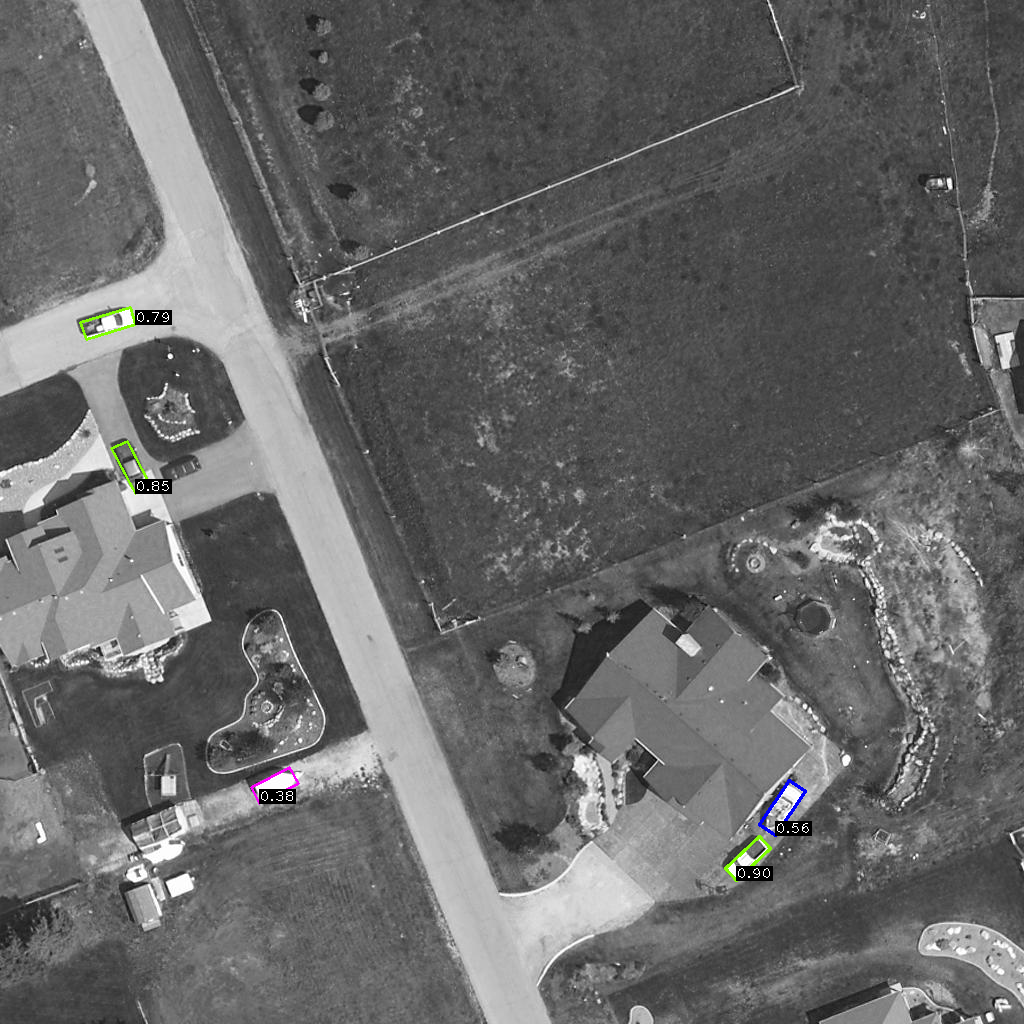
\includegraphics[width=\linewidth]{images/015Results/03ablation/comp_images/blue/509.png}
        \caption{Ship}
    \end{subfigure}
    \begin{subfigure}[t]{0.38\textwidth}
        \centering
        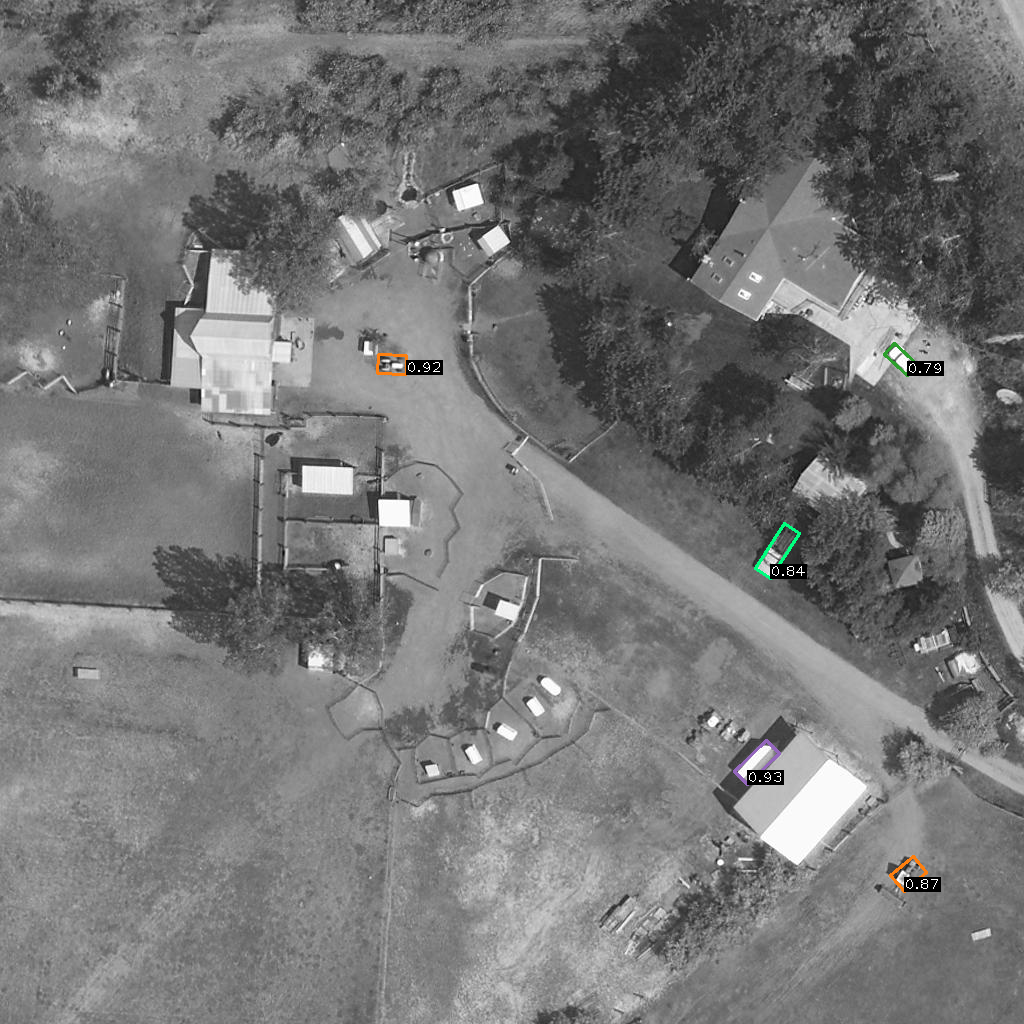
\includegraphics[width=\linewidth]{images/015Results/03ablation/comp_images/blue/523.png}
        \caption{Car, Tractor, Pick-Up}
    \end{subfigure}
    
    \caption[Blue Model – Full Sized Images]{Blue Model – Full Sized Images. The captions below the partial illustrations correspond to the classes shown in the example images. However, the illustrations generally show more classes than are indicated in the captions.}
    \label{fig:blue_ablation_examples_fs}
\end{figure}

\begin{figure}[h!]
    \centering
    \begin{subfigure}[t]{0.38\textwidth}
        \centering
        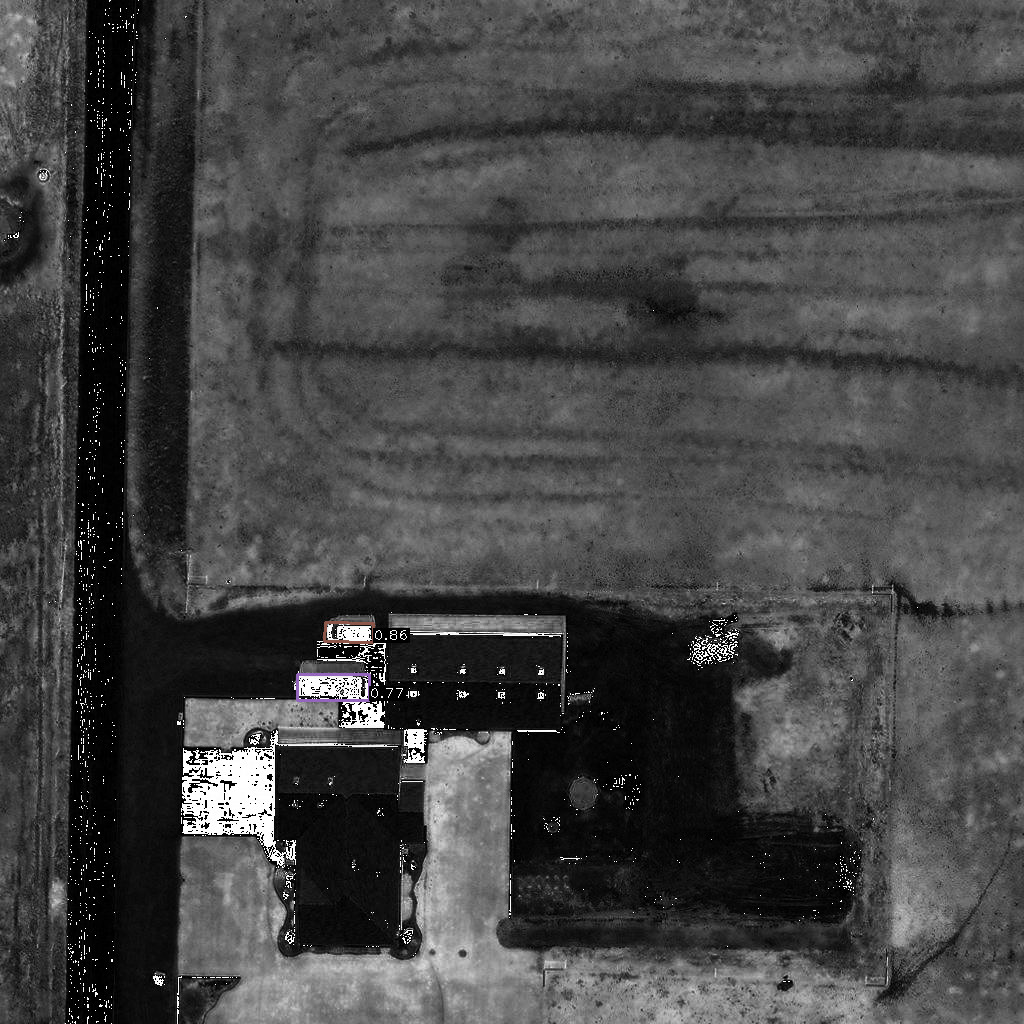
\includegraphics[width=\linewidth]{images/015Results/03ablation/comp_images/ndvi/198.png}
        \caption{Van}
    \end{subfigure}
    \begin{subfigure}[t]{0.38\textwidth}
        \centering
        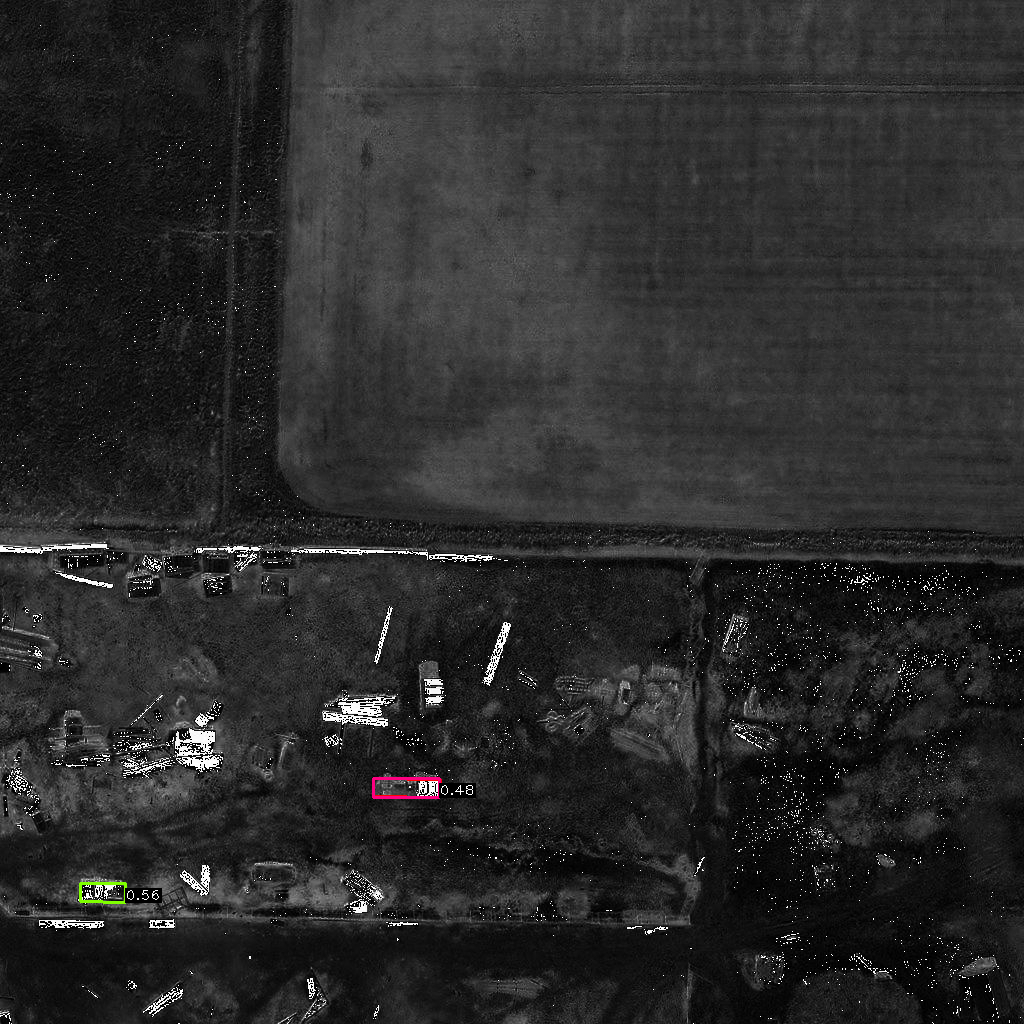
\includegraphics[width=\linewidth]{images/015Results/03ablation/comp_images/ndvi/212.png}
        \caption{Truck}
    \end{subfigure}
    
    \begin{subfigure}[t]{0.38\textwidth}
        \centering
        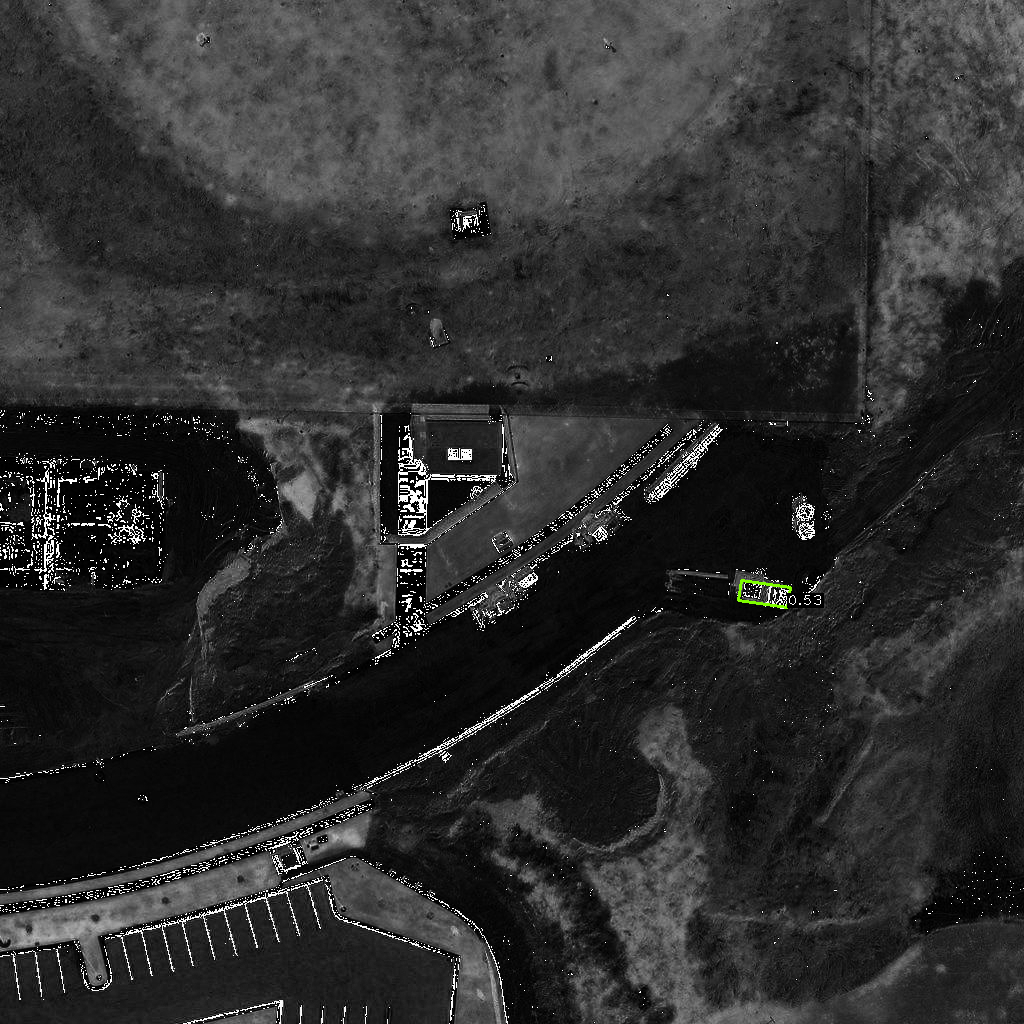
\includegraphics[width=\linewidth]{images/015Results/03ablation/comp_images/ndvi/427.png}
        \caption{Vehicle}
    \end{subfigure}
    \begin{subfigure}[t]{0.38\textwidth}
        \centering
        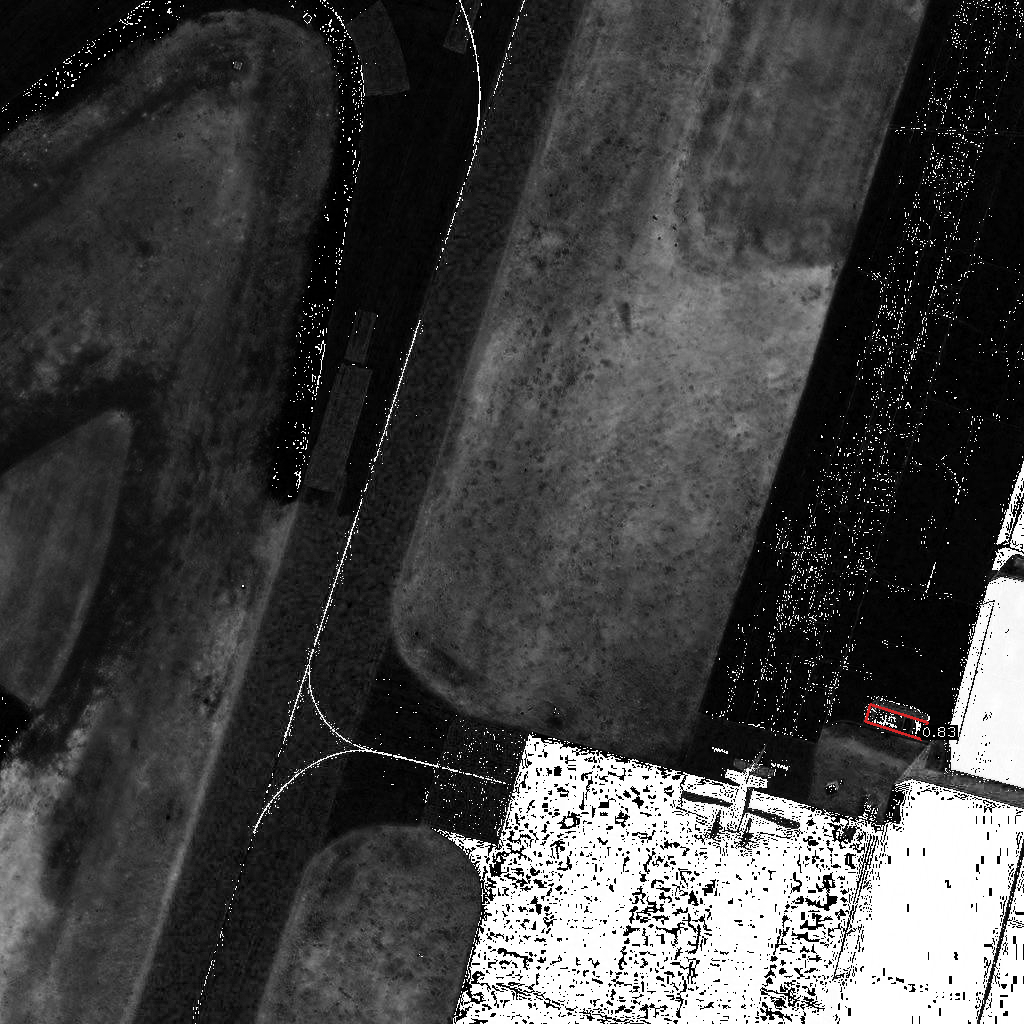
\includegraphics[width=\linewidth]{images/015Results/03ablation/comp_images/ndvi/487.png}
        \caption{Plane}
    \end{subfigure}
    
    \begin{subfigure}[t]{0.38\textwidth}
        \centering
        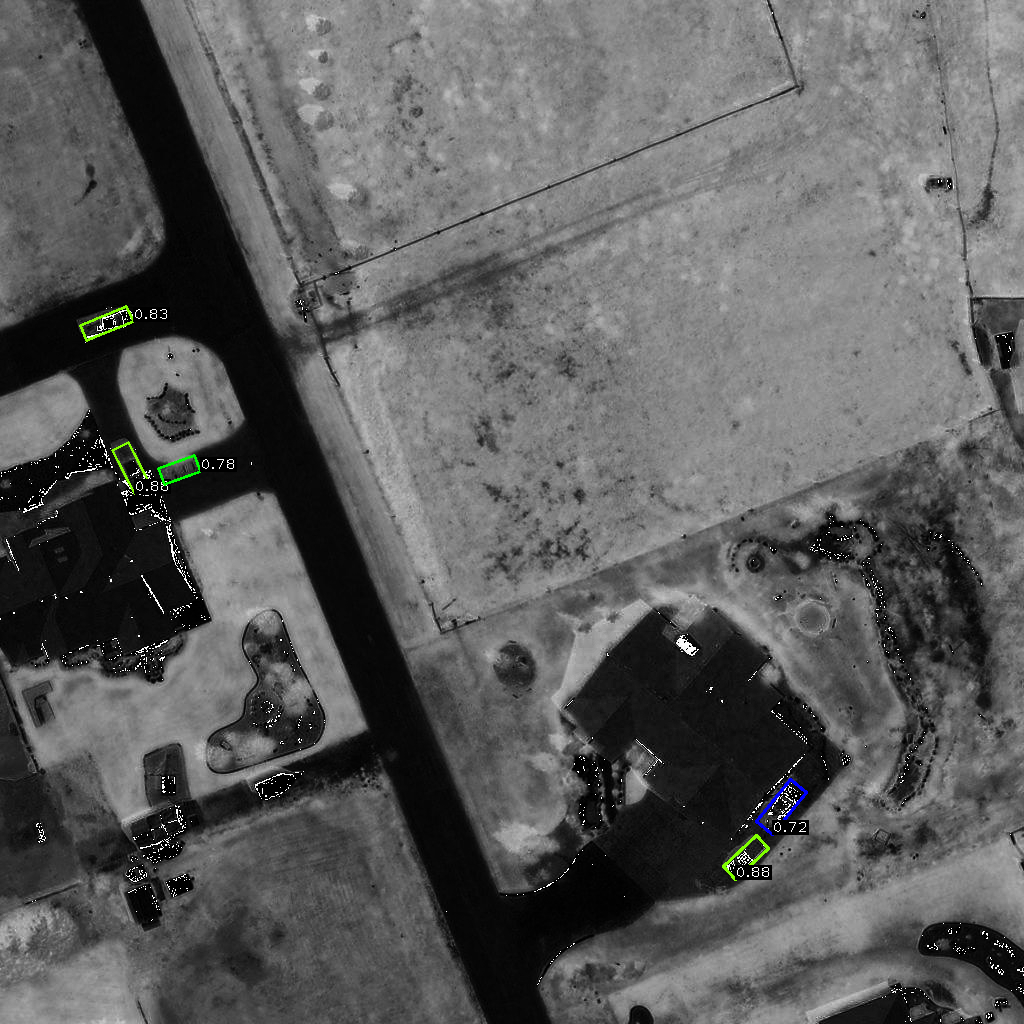
\includegraphics[width=\linewidth]{images/015Results/03ablation/comp_images/ndvi/509.png}
        \caption{Ship}
    \end{subfigure}
    \begin{subfigure}[t]{0.38\textwidth}
        \centering
        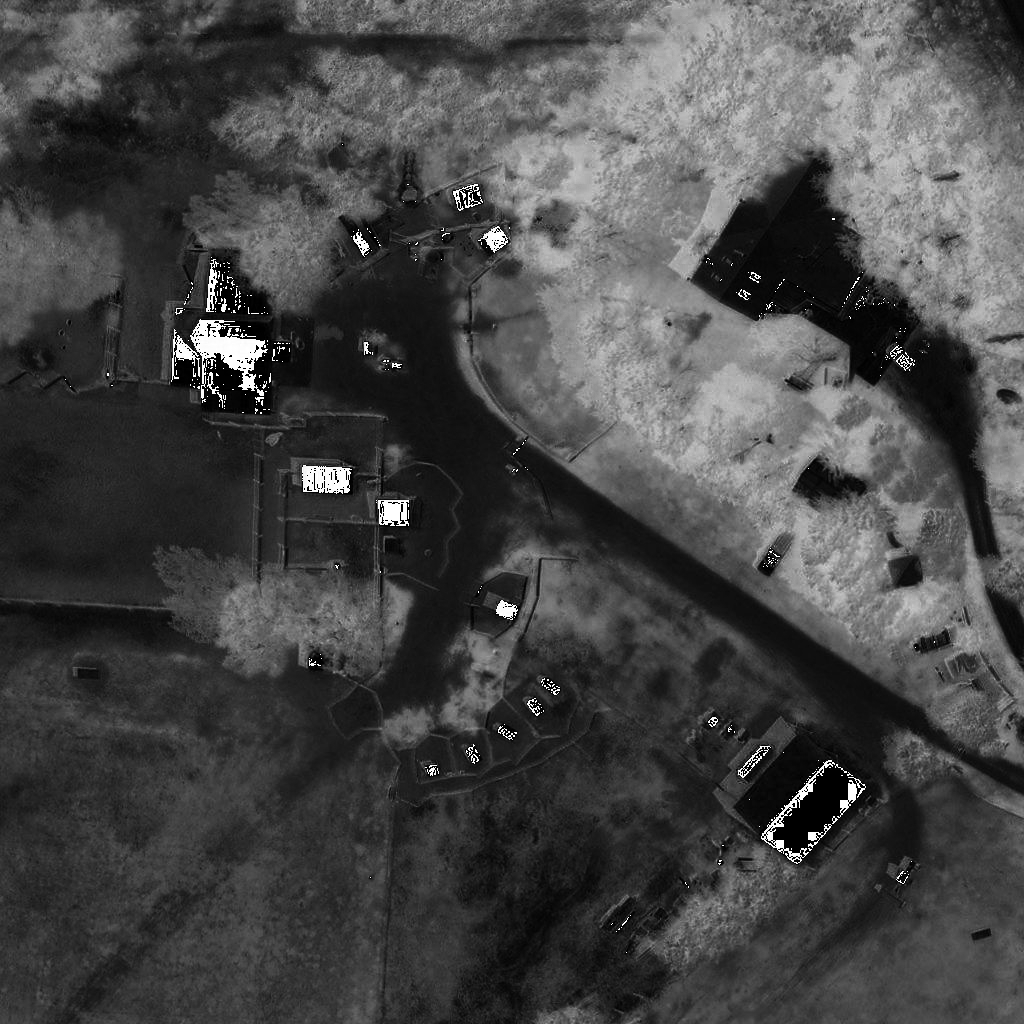
\includegraphics[width=\linewidth]{images/015Results/03ablation/comp_images/ndvi/523.png}
        \caption{Car, Tractor, Pick-Up}
    \end{subfigure}
    
    \caption[NDVI Model – Full Sized Images]{NDVI Model – Full Sized Images. The captions below the partial illustrations correspond to the classes shown in the example images. However, the illustrations generally show more classes than are indicated in the captions.}
    \label{fig:ndvi_ablation_examples_fs}
\end{figure}


